\section{Introduction}

Large language model (LLM) agents are increasingly equipped with external tools such as search engines, retrievers, calculators, and code interfaces. Such tool-using agents have shown promise in question answering, decision support, and interactive problem solving. However, practical agent systems often suffer from a persistent systems-level problem: better task performance usually requires more reasoning steps, more tool interactions, and longer execution trajectories, which in turn increase token usage and wall-clock latency.

Existing approaches typically fall into two broad categories. The first category uses fixed workflows, where the execution pipeline is manually specified in advance. These methods are stable and predictable, but they are often too rigid to adapt to task difficulty or changing intermediate evidence. The second category uses free-form agent reasoning, such as ReAct-style interaction loops, where the model repeatedly reasons, acts, and observes. These methods are more flexible and often stronger in task quality, but they can also incur unnecessary intermediate steps, repeated tool calls, and inflated execution cost.

This paper focuses on the following question: \emph{can agent behavior be controlled more explicitly, so that the trade-off between answer quality and execution cost becomes more analyzable and more controllable?} Instead of treating orchestration as an implicit consequence of prompting alone, we formulate it as an explicit decision problem. At each step, the agent chooses among actions such as answering directly, retrieving more evidence, invoking a tool, verifying current evidence, or stopping. We instantiate this idea with a utility-guided policy that scores candidate actions using heuristic signals including estimated gain, step cost, uncertainty, and redundancy.

Our contribution is not to propose a fully learned reinforcement learning policy, nor to claim universal superiority over all baselines. Rather, we make three more targeted contributions. First, we provide an explicit orchestration framework for tool-using LLM agents. Second, we analyze how different utility components affect the quality--cost trade-off. Third, we strengthen the empirical discussion through dedicated analyses of cost proxy design, workflow fairness, and redundancy control. These results show that explicit orchestration is a meaningful systems problem in its own right, and that even lightweight utility-guided control can offer useful structure for building more efficient and more interpretable agents.
These results show that explicit orchestration is a meaningful systems problem in its own right, and that even lightweight utility-guided control can offer useful structure for building more efficient and more interpretable agents.

Our implementation and experimental code are publicly available at \url{https://github.com/kagami-kasumi/Utility-Guided-Agent-Orchestration-for-Efficient-LLM-Tool-Use}.

\begin{figure}[t]
\centering
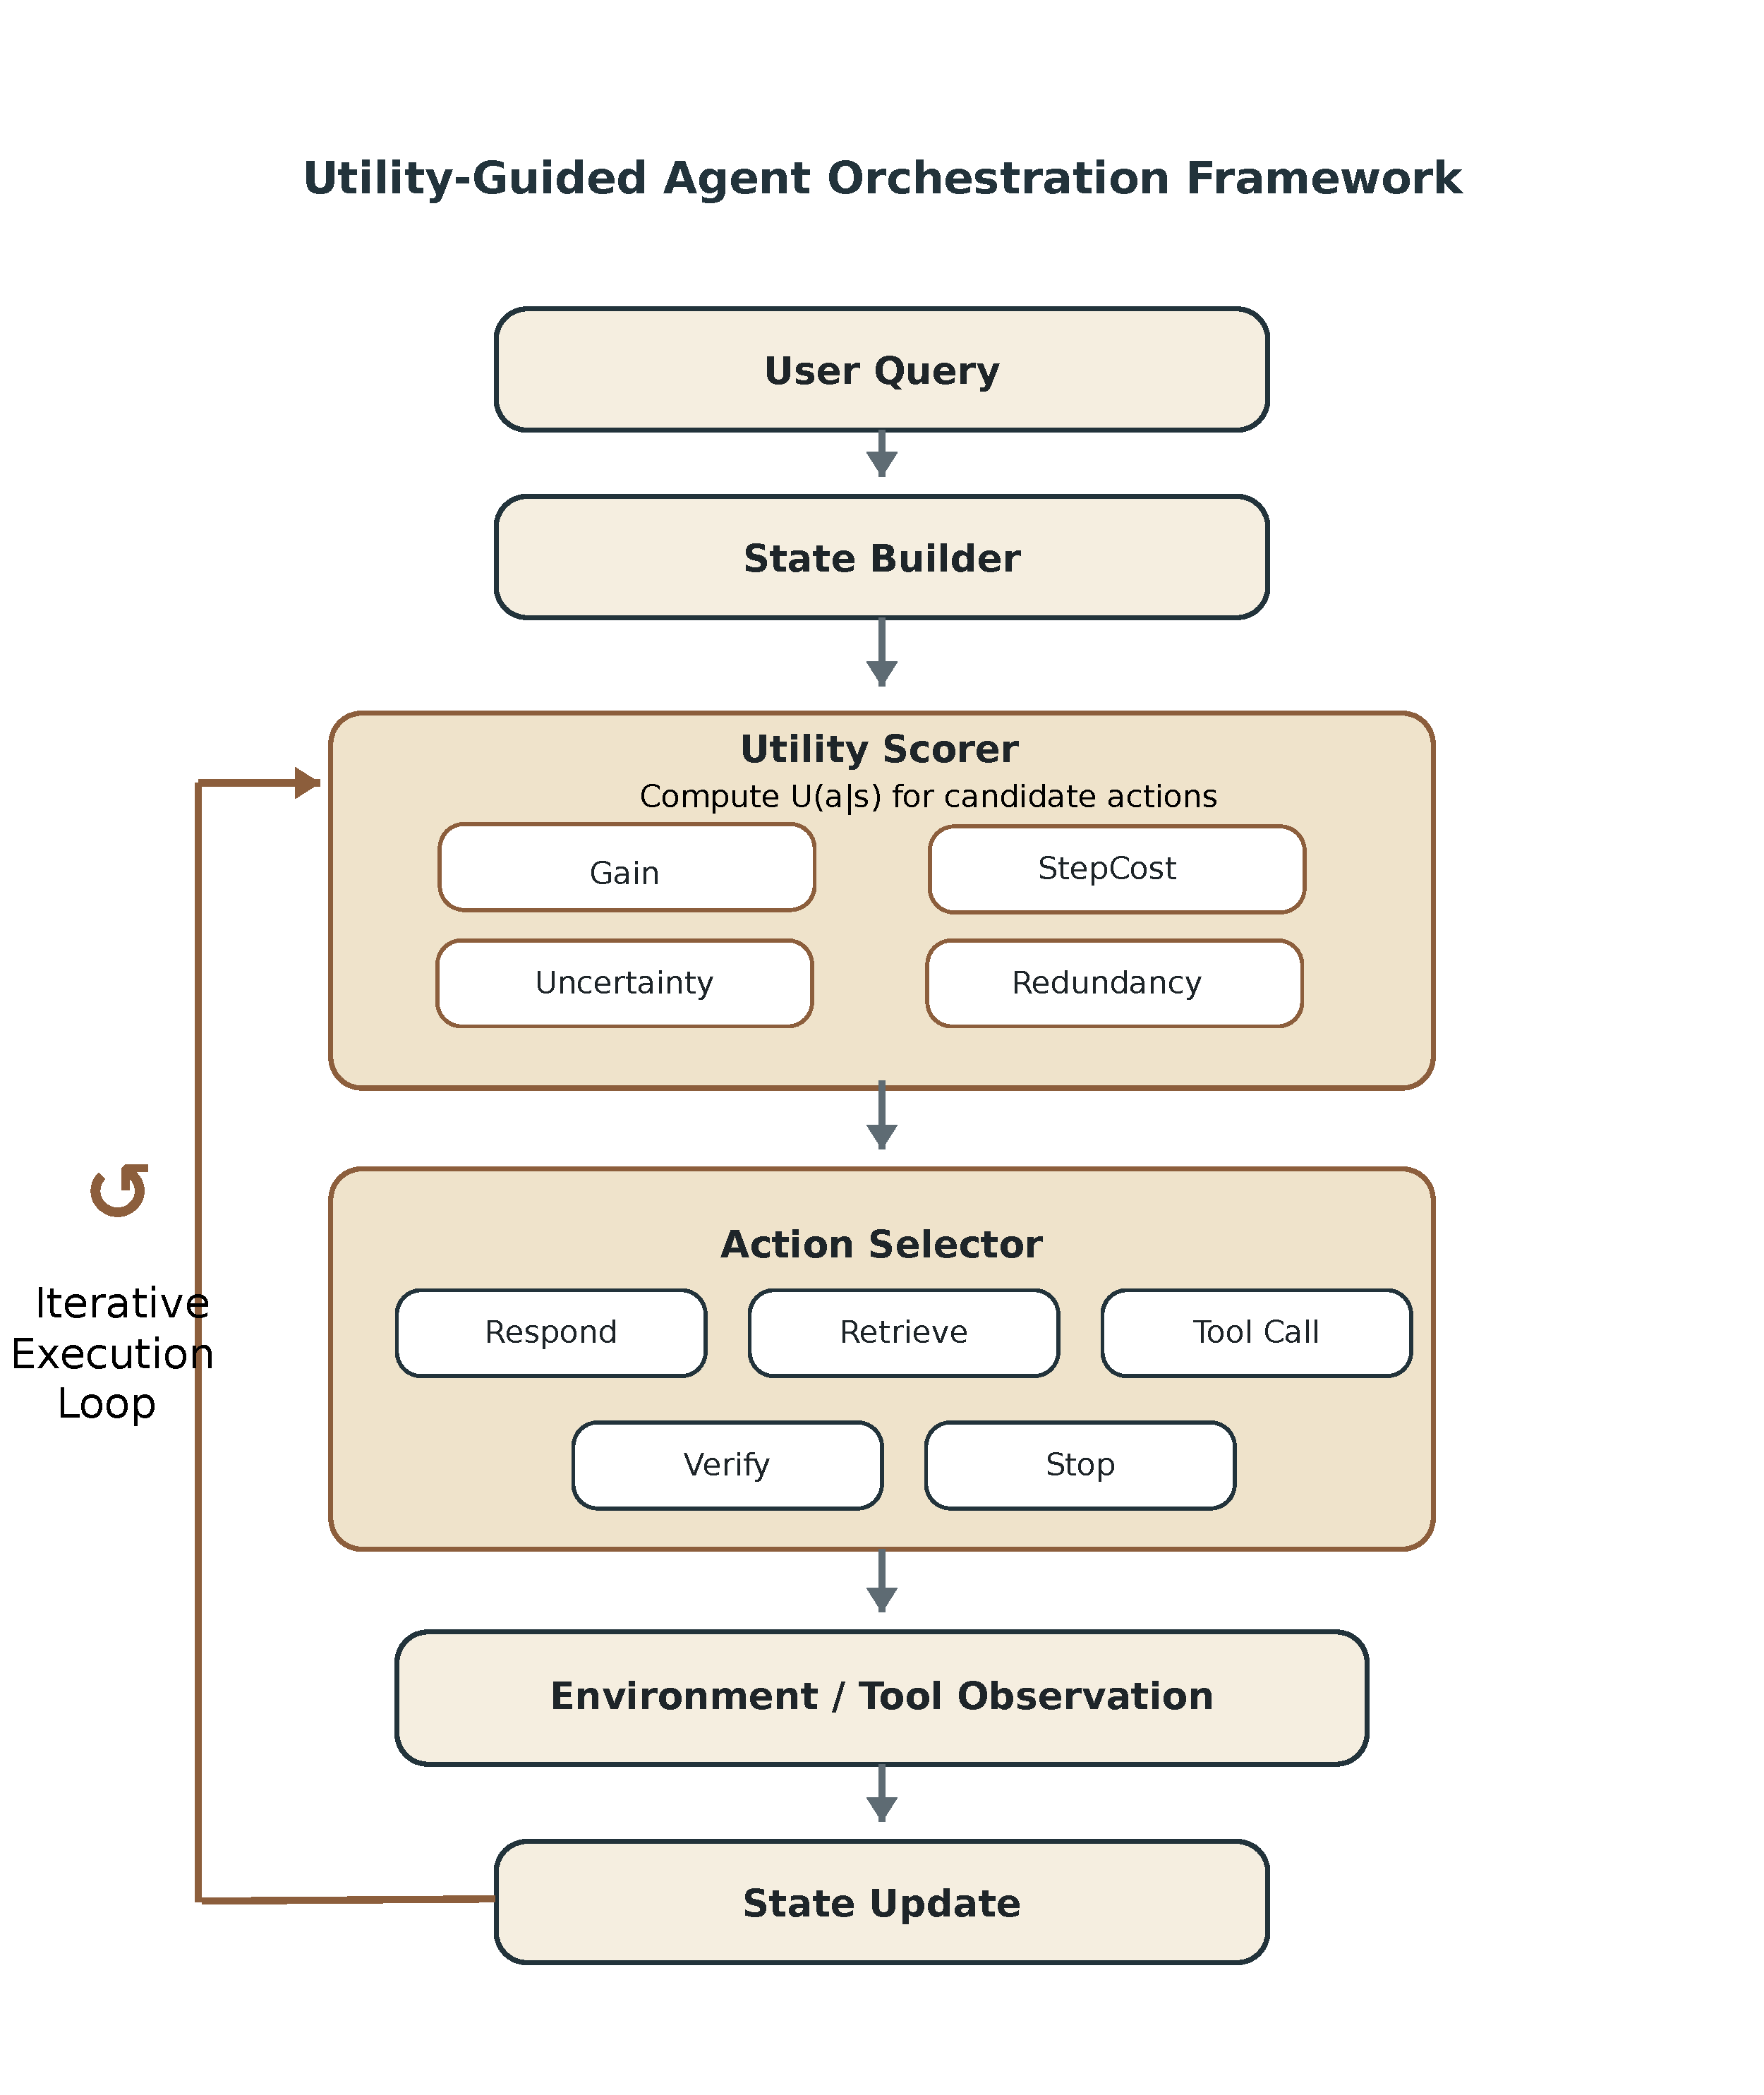
\includegraphics[width=120mm]{figures/overview.pdf}
\caption{
Overview of the proposed utility-guided agent orchestration framework.
At each step, the agent constructs a state representation from the current query, interaction history, and tool observations.
A utility scorer evaluates candidate actions using estimated gain, step cost, uncertainty, and redundancy, and the action selector chooses the highest-utility action.
The process iterates until a stopping condition is met.
}
\label{fig:framework}
\end{figure}
Figure~\ref{fig:framework} illustrates the overall architecture of the proposed framework.
